\documentclass{article}
\usepackage[utf8]{inputenc}
\usepackage{amsmath}
\usepackage{graphicx}
\graphicspath{ {images/} }

\title{Algoritmi di ordinamento a confronto}
\author{Marco Benelli}
\date{Settembre 2019}

\begin{document}

\maketitle

\section{Introduzione}

L'obiettivo è confrontare le velocità e le complessità di due algoritmi di ordinamento e verificare che queste siano coerenti con i risultati teorici.

\section{Teoria}

\subsection{Insertion sort}

Dallo studio teorico dell'algoritmo sappiamo che l'insertion sort ha un costo medio quadratico ($\Theta(n^2)$). Però sappiamo anche che nel caso migliore (ovvero quando l'array è già ordinata) ha un costo lineare ($\Theta(n)$).

\subsection{Merge sort}

Il merge sort è uno dei migliori algoritmi per quanto riguarda il tempo in quanto in qualunque caso (anche in quello peggiore) ha una complessità del tipo $\Theta(n \log(n))$.

\section{Prestazioni attese}

Le complessità di cui si è parlato nella sezione precedente sono da intendersi come asintotiche. I tempi di esecuzione possono avere un andamento diverso per array piccole. Quello che speriamo è che raggiungano un andamento simile a quello teorico anche per array relativamente piccole.

\section{Esperimenti}

Verranno svolti 4 esperimenti: 2 per l'insertion sort e 2 per il merge sort, 2 su array casuali e 2 su array già ordinate. Gli esperimenti verranno condotti su array di lunghezza sempre crescente (ogni volta la lunghezza viene raddoppiata) finché il tempo di esecuzione non supera i 128 secondi. Per ogni lunghezza e per ogni algoritmo vengono condotti 8 test e viene fatta la media fra i loro tempi di esecuzione.

\section{Codice}

Il codice è diviso in quattro sezioni: le funzioni che implementano gli algoritmi di ordinamento (queste sono semplicemente delle traduzioni in Python dello pseudo codice visto a lezione), le funzioni per la creazione delle array, le funzioni che implementano i test e le funzioni che disegnano i grafici.

Le funzioni per la generazione creano liste Python usando la funzione random per le array casuali.

Per misurare i tempi di esecuzione si usa la funzione default\_timer dal modulo timeit della libreria standard di Python.

Per quanto riguarda i grafici, si usa la libreria matplotlib, nello specifico il modulo pyplot. I vettori che vengono dati alla funzione plot sono il vettore delle lunghezze delle array (come vettore delle ascisse) e il vettore dei tempi di esecuzione (come vettore delle ordinate) per ogni test. Oltre a queste quattro curve (separate in due figure), vengono anche disegnate altre quattro curve che simboleggiano l'andamento predetto dalla teoria per confrontarlo con l'andamento sperimentale.

\section{Risultati sperimentali}

\begin{figure}[ht]
    \centering
    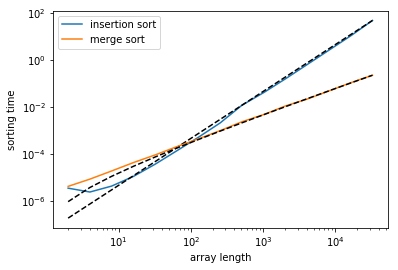
\includegraphics{random}
    \caption{Il grafico del test su array casuali. L'insertion sort ha una complessità quadratica, mentre il merge sort ha una complessità del tipo $n\log(n)$}
    \label{fig:random}
\end{figure}

\begin{figure}[ht]
    \centering
    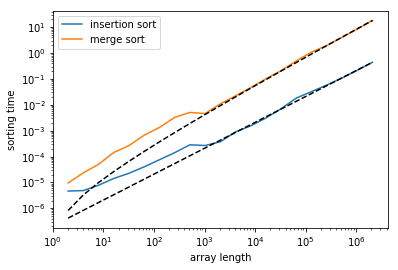
\includegraphics{sorted}
    \caption{Il grafico del test su array ordinate. In questo caso l'insertion sort ha una complessità lineare, mentre il merge sort continua ad avere complessità $n\log(n)$}
    \label{fig:sorted}
\end{figure}

Nelle figure \ref{fig:random} e \ref{fig:sorted} possiamo vedere che i risultati sperimentali sono in linea con le predizioni teoriche visto che le linee colorate si sovrappongono a quelle tratteggiate. È importante notare che i grafici sono in scala logaritmica, in modo che complessità lineari e complessità quadratiche possano essere rappresentate con una retta. Le linee tratteggiate indicano l'andamento teorico e sono ottenute moltiplicando la funzione teorica per un coefficiente opportuno. Questo coefficiente si trova imponendo che la linea tratteggiata e quella colorata abbiano in comune l'ultimo punto.

Questi risultati ci portano a concludere che il merge sort è migliore dell'insertion sort nella maggior parte delle applicazioni. Tuttavia anche il merge sort ha dei problemi per array troppo lunghe: lo spazio occupato è lineare rispetto alla lunghezza dell'array. Per questo motivo in certi casi si potrebbe preferire un'altro algoritmo.

\end{document}
